\chapter{Themis: I/O-Efficient MapReduce}
\label{chapter:themis}

This chapter presents Themis, an I/O-efficient MapReduce system derived from
TritonSort. Themis is named after the Titan in Greek mythology who is tasked
with creating balance, order and harmony.

Many MapReduce jobs are I/O-bound, and so minimizing the number of I/O
operations is critical to improving their performance. Themis reads and writes
data records to disk exactly twice, which is the minimum amount possible for
data sets that cannot fit in memory.

In order to minimize I/O, Themis makes fundamentally different design decisions
from previous MapReduce implementations. Themis performs a wide variety of
MapReduce jobs -- including click log analysis, short-read sequence alignment,
and PageRank -- at nearly the speed of TritonSort's record-setting sort
performance.

\section{Introduction}
\label{themis:sec:intro}

Our experience building TritonSort shows that an appropriately balanced
implementation can realize orders of magnitude improvement in throughput and
efficiency.  Translating these types of gains to more general-purpose data
processing systems will help close the efficiency gap present in modern
large-scale data processing systems, allowing more work to be performed with
the same hardware, or the same amount of work to be performed with less
hardware. This improved efficiency will result in substantially lowered system
cost, energy usage, and management complexity.

Given that many MapReduce jobs are I/O-bound, an efficient MapReduce system
must aim to minimize the number of I/O operations it performs.  Fundamentally,
every MapReduce system must perform at least two I/O operations per record when
the amount of data exceeds the amount of memory in the cluster~\cite{sort-io}.
We refer to a system that meets this lower-bound as having the ``2-IO''
property.  Any data processing system that does not have this property is doing
more I/O than it needs to.  Existing MapReduce systems incur additional I/O
operations in exchange for simpler and more fine-grained fault tolerance.

Themis is an implementation of MapReduce designed to have the 2-IO
property. Themis accommodates the flexibility of the MapReduce programming
model while simultaneously delivering high efficiency.  It does this by
considering fundamentally different points in the design space than existing
MapReduce implementations:

\paragraph{1. Eliminating task-level fault tolerance:} At the scale of tens of
thousands of servers, failures are common, and so MapReduce was designed with a
strong task-level fault tolerance model.  However, more aggressive fault
tolerance gains finer-grained restart at the expense of lower overall
performance.  Interestingly, many Hadoop users report cluster sizes of under
100 nodes~\cite{HadoopPoweredBy}, much smaller than those deployed by
MapReduce's early adopters.  In 2011, Cloudera's VP of Technology Solutions
stated that the mean size of their clients' Hadoop clusters is 200 nodes, with
the median size closer to 30~\cite{MonashTrajman}.  At this moderate scale,
failures are much less common, and aggressive fault tolerance is wasteful in
the common case.  Foregoing task-level fault tolerance permits a design that
achieves the 2-IO property.  When a job experiences a failure, Themis simply
re-executes it.  This optimistic approach to fault tolerance enables Themis to
aggressively pipeline record processing without unnecessarily materializing
intermediate results to disk.  As we will show in
Chapter~\ref{chapter:fault_tolerance}, for moderate cluster sizes this approach
has the counter-intuitive effect of improving performance despite the
occasional job re-execution.

\paragraph{2. Dynamic, adaptive memory allocation:} To maintain the 2-IO
property, Themis must process a record completely once it is read from disk.
This prevents Themis from putting records back on disk in response to memory
pressure through swapping or writing spill files.  Themis implements a
policy-based, application-level memory manager that provides fine-grained
sharing of memory between operators processing semi-structured, variably-sized
records.  This allows it to support datasets with as much as a factor of
$10^7$ skew between record sizes while maintaining the 2-IO property.

\paragraph{3. Central management of shuffle and disk I/O:} Themis uses a
centralized, per-node disk scheduler that ensures that records from multiple
sources are written to disk in large batches to reduce disk seeks.  Themis
delivers nearly sequential disk I/O across a variety of MapReduce jobs, even
for workloads that far exceed the size of main memory.

To validate our design, we have written a number of MapReduce programs on
Themis, including a web user session tracking application, PageRank, n-gram
counting, and a DNA read sequence alignment application.  We found that Themis
processes these jobs at nearly the per-node performance of TritonSort's
record-setting sort run and nearly the maximum sequential speed of the
underlying disks.

\section{The Challenge of Skew}
\label{themis:sec:challenges}

One of MapReduce's attractive properties is its ability to handle
semi-structured and variably-sized data.  This variability makes maintaining
the 2-IO property a challenge.  In this section, we describe two sources of
variability and the resulting requirements they place on our design.

An input dataset can exhibit several different kinds of \emph{skew},
which simply refers to variability in its structure and content.  These
include:

\paragraph{Record Size Skew:} In systems with semi-structured or unstructured
data, some records may be much larger than others.  This is called \emph{record
  size skew}.  In extreme cases, a single record may be gigabytes in size.

\paragraph{Partitioning Skew:} Data that is
not uniformly distributed across its keyspace exhibits \emph{partitioning
  skew}.  This can cause some nodes to process much more data than others if
the data is na\"{\i}vely partitioned across nodes, creating
stragglers~\cite{DeWittGraySkew}.  Handling skew in MapReduce is complicated by
the fact that the distribution of keys in the data produced by a \map function
is often not known in advance.  Existing MapReduce implementations handle
partitioning skew by spilling records to disk that cannot fit into memory.

\paragraph{Computational Skew:} In a dataset exhibiting
\emph{computational skew}, some records take much longer than average to
process.  Much of the work on mitigating computational skew in MapReduce
involves exploiting the nature of the particular problem and relying on a
degree of user guidance~\cite{SkewReduce} or proactively re-partitioning
the input data for a task~\cite{SkewTune}.  As the focus of our work is
I/O-bound jobs, we do not consider computational skew in this work.

\paragraph{Performance Heterogeneity:} The performance of a
population of identical machines can vary significantly; the reasons for this
heterogeneity are explored in \cite{stutterfault}. In addition, clusters are
rarely made up of a homogeneous collection of machines, due both to machine
failures and planned incremental upgrades. While we believe that the techniques
presented in this work can be applied to heterogeneous clusters, we have not
evaluated Themis in such a setting.

To handle record skew, Themis dynamically controls its memory usage, which we
describe in Section~\ref{sec:memory}.  Themis adopts a sampling-based skew
mitigation technique to minimize the effects of partitioning skew.  We discuss
this mitigation technique in Section~\ref{sec:phase_zero}.

\section{System Architecture}
\label{sec:design}

In this section, we describe the design of Themis.

\subsection{Core Architecture}
\label{sec:overview}

Themis reuses several core runtime components that were used to build
TritonSort.  Like TritonSort, Themis is written as a sequence of
\emph{phases}, each of which consists of a directed dataflow graph of
\emph{stages} connected by FIFO queues.  Each stage consists of a number of
\emph{workers}, each running as a separate thread.

\subsection{MapReduce Overview}

\begin{figure*}
\centering
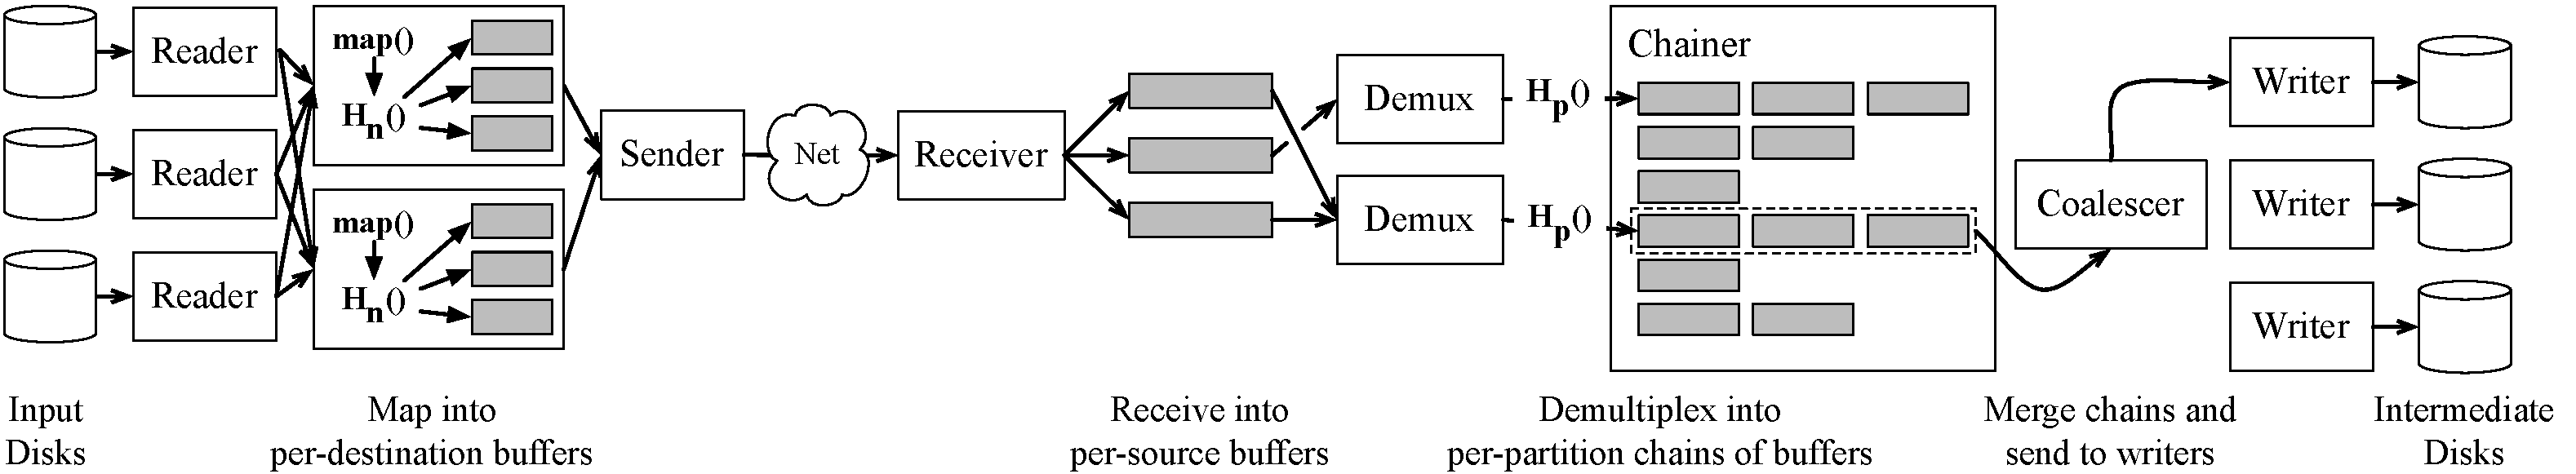
\includegraphics[width=\textwidth]{themis/figures/detailed_phase_one.pdf}
\caption{\label{fig:phase_one} Stages of Phase One (Map/Shuffle) in Themis}
\end{figure*}

Unlike existing MapReduce systems, which executes \map and \reduce tasks
concurrently in waves, Themis implements the MapReduce programming model in
three phases of operation, summarized in Table~\ref{tbl:stages}.  Phase zero,
described in Section~\ref{sec:phase_zero}, is responsible for sampling input
data to determine the distribution of record sizes as well as the distribution
of keys.  These distributions are used by subsequent phases to minimize
partitioning skew.  Phase one, described in Section~\ref{sec:phase_one}, is
responsible for applying the \map function to each input record, and routing
its output to an appropriate partition in the cluster.  This is the equivalent
of existing systems' map and shuffle phases.  Phase two, described in
Section~\ref{sec:phase_two}, is responsible for sorting and applying the
\reduce function to each of the intermediate partitions produced in phase one.
At the end of phase two, the MapReduce job is complete.

\begin{table}
\centering
\caption{\label{tbl:stages} Themis's three stage architecture}
\begin{tabular}{|c|c|c|} \hline
\textbf{Phase} & \textbf{Description} & \textbf{Required?} \\\hline
0 & Skew Mitigation & Optional \\
1 & \texttt{map()} and shuffle & Required \\
2 & sort and \texttt{reduce()} & Required \\\hline
\end{tabular}
\end{table}

Phase one reads each input record and writes each intermediate record exactly
once.  Phase two reads each intermediate partition and writes its corresponding
output partition exactly once.  Thus, Themis has the 2-IO property.

\subsection{Phase One: Map and Shuffle}
\label{sec:phase_one}
\label{sec:map}

Phase one is responsible for implementing both the \map operation as well as
shuffling records to their appropriate intermediate partition.  Each node in
parallel implements the stage graph pipeline shown in
Figure~\ref{fig:phase_one}.

The \Readerbf stage reads records from an input disk and sends them to the
\Mapperbf stage, which applies the \map function to each record.  As the \map
function produces intermediate records, each record's key is hashed to
determine the node to which it should be sent and placed in a
per-destination buffer that is given to the \sender when it is full.  The
\Senderbf sends data to remote nodes using a round-robin loop of short,
non-blocking \texttt{send()} calls.  We call the \Reader to \Sender part of the
pipeline the ``producer-side'' pipeline.

The \Receiverbf stage receives records from remote nodes over TCP using
a round-robin loop of short, non-blocking \texttt{recv()} calls. We implemented
a version of this stage that uses \texttt{select()} to avoid unnecessary
polling, but found that its performance was too unpredictable to reliably
receive all-to-all traffic at 10Gbps. The \receiver places incoming records
into a set of small per-source buffers, and sends those buffers to
the \Demux stage when they become full.

The \Demuxbf stage is responsible for assigning records to partitions.  It
hashes each record's key to determine the partition to which it should be
written, and appends the record to a small per-partition buffer.  When that
buffer becomes full, it is emitted to the \Chainerbf stage, which links buffers
for each partition into separate \emph{chains}.  When chains exceed a
pre-configured length, which we set to 4.5 MB to avoid doing small writes, it
emits them to the \Coalescerbf stage.  The \Coalescerbf stage merges chains
together into a single large buffer that it sends to the \Writerbf stage,
which appends buffers to the appropriate partition file. The combination of the
\Chainer and \Coalescer stages allows buffer memory in front of the \Writer
stage to be allocated to partitions in a highly dynamic and fine-grained way.
We call the \Receiver to \Writer part of the pipeline the ``consumer-side''
pipeline.

A key requirement of the consumer-side pipeline is to perform large, contiguous
writes to disk to minimize seeks and provide high disk bandwidth.  Themis uses
the same node-wide, application-driven disk scheduler used in TritonSort to
ensure that writes are large. We refer the reader to
Section~\ref{sec:tritonsort-disk-scheduler} for details on the disk scheduler's
implementation.

\subsection{Phase Two: Sort and Reduce}
\label{sec:phase_two}
\label{sec:reduce}

\begin{figure}[h]
\centering

\includegraphics[width=\columnwidth]{themis/figures/phase_two.pdf}
\caption{\label{fig:phase_two} Stages of Phase Two (Sort/Reduce) in Themis}
\end{figure}

By the end of phase one, the map function has been applied to each input
record, and the records have been grouped into partitions and stored on the
appropriate node so that all records with the same key are stored in a single
partition.  In phase two, each partition must be sorted by key, and the \reduce
function must be applied to groups of records with the same key.  The stages
that implement phase two are shown in Figure~\ref{fig:phase_two}.

There is no network communication in phase two, so nodes process their
partitions independently.  Entire partitions are read into memory at once by
the \Readerbf stage. A \Sorterbf stage sorts these partitions by key, keeping
the result in memory.  The \Reducerbf stage applies the \reduce function to all
records sharing a key.  Reduced records are sent to the \Writerbf, which writes
them to disk.

All records with a single key must be stored in the same partition for the
\reduce function to produce correct output. As a result, partitioning skew can
cause some partitions to be significantly larger than others. Themis's memory
management system allows phase two to process partitions that approach the size
of main memory, and its optional skew mitigation phase can reduce partitioning
skew without user intervention. We describe these systems in Sections
\ref{sec:memory} and \ref{sec:phase_zero}, respectively.

A key feature of Themis's \sorter stage is that it can select which sort
algorithm is used to sort a buffer on a buffer-by-buffer basis.  There is a
pluggable \textit{sort strategy} interface that lets developers use different
sorting algorithms; currently quicksort and radix sort are implemented.  Each
sort strategy calculates the amount of scratch space it needs to sort the given
buffer, depending on the buffer's contents and the sort algorithm's space
complexity.  For both quicksort and radix sort, this computation is
deterministic.  In Themis, radix sort is chosen if the keys are all the same
size and the required scratch space is under a configurable threshold;
otherwise, quicksort is used.

\section{Memory Management and Flow Control}
\label{sec:memory}

\begin{table}
  \centering
  \caption{\label{fig:memory-allocator-compare} A comparison of Themis's memory
    allocator implementations.}
  \tabcolsep=0.11cm

  \begin{tabular}{|c|c|c|p{.7cm}|p{.7cm}|p{.7cm}|c|} \hline
    & \multirow{2}{*}{\textbf{TritonSort}} & \multirow{2}{*}{\textbf{Themis}}
    & \multicolumn{3}{c|}{\textbf{Used in Phase}} & \textbf{Subject to} \\\cline{4-6}
    & & & \centering 0 & \centering 1 & \centering 2 & \textbf{deadlock?} \\ \hline
    Pool & $\checkmark$ & $\checkmark$ & \centering $\checkmark$ & \centering $\checkmark$ & & \\\hline
    Quota &  & $\checkmark$ & \centering $\checkmark$ & \centering $\checkmark$ & &  \\\hline
    Constraint &  & $\checkmark$ &  &  & \centering $\checkmark$ & $\checkmark$ \\\hline
  \end{tabular}
\end{table}

Themis relies on a dynamic and flexible memory management system
to partition memory between operators.
Themis's memory manager actually serves two distinct purposes: (1) it
enables resource sharing between operators, and (2) it supports
enforcing back-pressure and flow control.  In the first case, Themis requires
flexible use of memory given our desire to support large amounts of record
size
skew while maintaining the 2-IO property.  In the second case, individual
stages in the Themis pipeline naturally run at different speeds (e.g.,
the network is 10 Gbps, whereas the disk subsystem only supports writing
at approximately 5.5 Gbps), and so back-pressure and flow control are needed
to prevent faster stages from starving slower stages for resources.

Themis supports a single memory allocation interface with pluggable memory
policies.  We first describe the memory allocator's interface, and then
describe the three policies that we have implemented.

\subsection{Memory Allocation Interface}

Worker stages in Themis allocate space for buffers and other necessary
scratch space using a unified and simple memory allocator interface,
shown in Table~\ref{fig:memory-allocator-API}.

\begin{table*}
  \centering
  \caption{\label{fig:memory-allocator-API} A summary of the Themis memory
    allocator API.}
  \resizebox{\columnwidth}{!}{
  \begin{tabular}{|l|l|}
    \hline
    \textbf{Function} & \textbf{Description} \\
    \hline
    \texttt{CallerID \textbf{registerCaller}(Worker worker)} & Register \texttt{worker}
    with the allocator \\
    \hline
    \texttt{void* \textbf{allocate}(CallerID caller, uint64\_t size)} & allocate a
    memory region of \texttt{size} bytes for \texttt{caller} \\
    \hline
    \texttt{void \textbf{deallocate}(void* memory)} & deallocate \texttt{memory} that
    was allocated by this allocator\\
    \hline
  \end{tabular}
  }
\end{table*}

Memory allocators can be assigned on a stage-by-stage basis, but in the current
implementation we assume that memory regions are allocated and deallocated by
the same allocator.  The \texttt{allocate} call blocks until the underlying
memory allocation policy satisfies the allocation, which can be an unbounded
amount of time.  As we will see, this simple mechanism, paired with one of
three memory policies, provides for both resource sharing as well as flow
control.  We now examine each of these polices.

\subsection{Policy 1: Pool-Based Management}

\begin{figure}
  \centering
  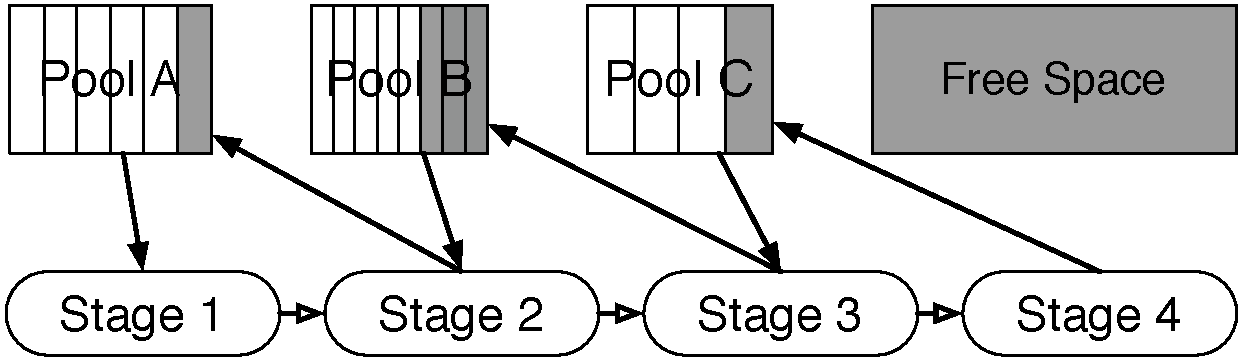
\includegraphics[width=\columnwidth]{themis/figures/pool_based_manager.pdf}
  \caption{\label{fig:memory_allocators:pool} A diagrammatic overview of
    pool-based memory management. Note that memory in each pool is divided into
  fixed-size regions, and that any memory not allocated to pools cannot be
  utilized by stages.}
\end{figure}

The first policy we consider is a ``pool'' memory policy, which is inherited
from TritonSort~\cite{tritonsort}.  A memory pool is a set of pre-allocated
buffers that is filled during startup.  Buffers can be checked out from a pool,
and returned when they are finished being used as illustrated in
Figure~\ref{fig:memory_allocators:pool}.  When a worker tries to check out a
buffer from an empty pool, it blocks until another worker returns a buffer to
that pool.  The pool memory policy has the advantage that all memory allocation
is done at startup, avoiding allocation during runtime.  Through efficient
implementation, the overhead of checking out buffers can be very small.  This
is especially useful for stages that require obtaining buffers with very low
latency, such as the \Receiver stage, which obtains buffers to use in receiving
data from the network.  The \receiver receives uninterpreted bytes from network
sockets into small, fixed-size byte buffers.  These buffers are passed to a
subsequent stage, which converts them into buffers containing complete records.
For this reason, the \receiver can use pool-based management while still
supporting record-size skew.

Pools can be used to provide resource sharing between workers by giving each of
those workers a reference to a single pool.  The producer-consumer relationship
between pairs of stages also provides a form of flow control; the upstream
stage checking out buffers can only produce work at the rate at which the
downstream stage can return them to the pool.  However, pools have several
disadvantages.  First, the buffers in a pool are all fixed-size, and so
the pool memory policy supports very limited amounts of data skew.  By
carving memory up into fixed-size pools, the maximum record size supported by
this policy is limited to the size of the smallest pool.  Additionally, buffer
pools reserve a fixed amount of memory for a particular pair of stages. One
consequence of this is a loss of flexibility; if one stage temporarily needs
more memory than usual (e.g., if it is handling a large record), it cannot
``borrow'' that memory from another stage due to the static partitioning of
memory across pools.

\subsection{Policy 2: Quota-Based Management}

\begin{figure}
  \centering
  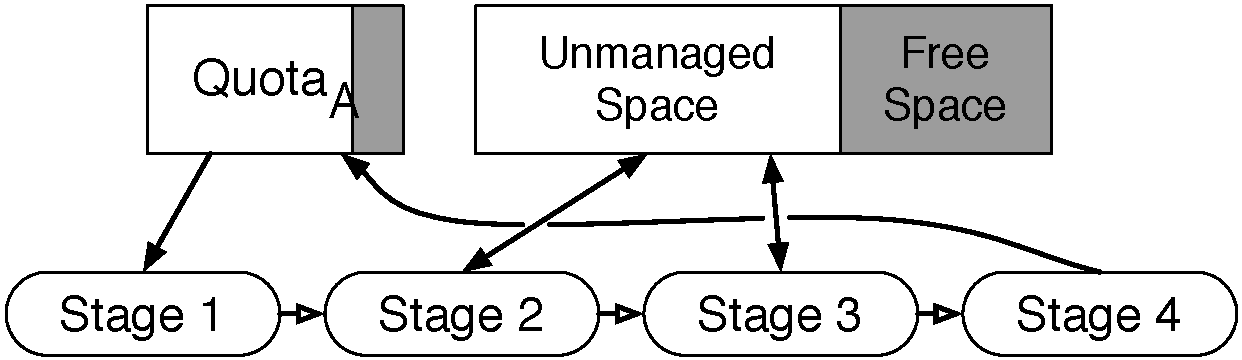
\includegraphics[width=\columnwidth]{themis/figures/quota_based_manager.pdf}
  \caption{\label{fig:memory_allocators:quota} A diagrammatic overview of
    quota-based memory management. In this figure, $Quota_A$ provides a memory
    quota between Stage 1 and Stage 4. Stages 2 and 3 use unmanaged memory
    created with standard \texttt{malloc} and \texttt{free} syscalls.}
\end{figure}

While the pool memory policy is simple, it is quite inflexible, and does not
handle skewed record sizes very well.  The quota-based memory policy is
designed to support more flexible memory allocation while still providing flow
control.  At a high level, the quota policy ensures that stages producing
records do not overwhelm stages that eventually consume them.  For example,
most of our evaluation is \writer limited, and so we want to ensure that the
\receiver stage, which produces records received from the network, does not
overwhelm the \writer stage, which is the bottleneck.

Themis has three such producer-consumer pairs: between the \reader and the
\mapper (with the \mapper acting as the consumer), between the \mapper and the
\sender (with the \mapper acting as the producer), and between the \receiver
and the \writer. The mapper acts as both a consumer and a producer, since it is
the only stage in the phase one pipeline that creates records as directed by
the \map function that were not read by the \reader.

Quotas are enforced by the queues between stages. A quota can be viewed as the
amount of memory that the pipeline between a producer and a consumer can use.
When a producer stage pushes a buffer into the pipeline, the size of that
buffer is debited from the quota.  When a consumer stage consumes that buffer,
the buffer's size is added back to the quota.  If a producer is about to exceed
the quota, then it blocks until the consumer has consumed sufficient
memory. Quota-based allocation is illustrated in
Figure~\ref{fig:memory_allocators:quota}.

Quota-based memory management dramatically reduces the number of variables that
need to be tuned relative to the pool-based memory policy.  One need only
adjust the quota allocations present between pairs of stages, rather than the
capacity of a much larger number of buffer pools.  Additionally, stages that
are not producers and consumers do not need to do any form of coordination,
which makes their memory allocations very fast.

Quota-based management assumes that any scratch space or additional memory
needed by stages between the producer and consumer is accounted for in the
quota.  This is to prevent intermediate stages from exceeding the total amount
of memory, since their memory accesses are not tracked.  It also tacitly
assumes that the size of a buffer being produced cannot exceed the size of the
quota. This is much less restrictive than a pool-based approach, as quotas are
typically several gigabytes.

\subsection{Policy 3: Constraint-Based Management}

\begin{figure}
  \centering
  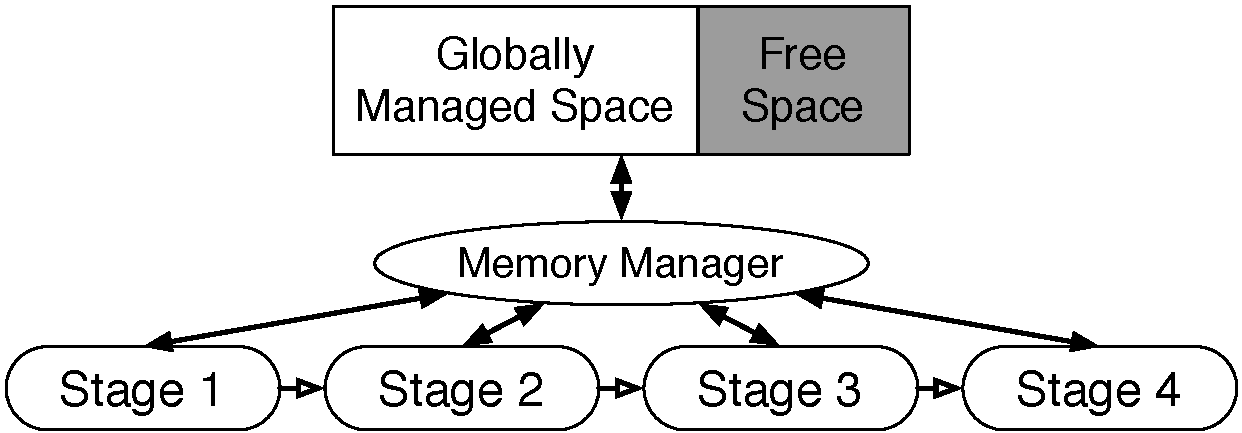
\includegraphics[width=\columnwidth]{themis/figures/constraint_based_manager.pdf}
  \caption{\label{fig:memory_allocators:constraint} A diagrammatic overview of
    constraint-based memory management. All stages' memory requests are
    satisfied by a central memory manager that schedules these requests
    according to the stage graph's structure.}
\end{figure}

In situations where the amount of memory used by stages to process records
cannot be determined in advance, quota-based systems are not ideal for
providing flow control. In these situations, Themis uses a more heavyweight,
constraint-based memory management policy.

In the constraint-based memory policy, the total amount of memory in use by
workers is tracked centrally in the memory allocator. If a worker requests
memory, and enough memory is available, that request is granted immediately.
Otherwise, the worker's request is added to a per-worker queue of outstanding
requests and the worker sleeps on a condition variable until the request can be
satisfied. Constraint-based allocation is illustrated in
Figure~\ref{fig:memory_allocators:constraint}.

When multiple workers have outstanding unsatisfied allocation requests, the
memory allocator prioritizes worker requests based on a worker's distance in
the stage graph to a stage that consumes records.  The producer-side pipeline
measures distance to the \sender stage, and the consumer-side pipeline measures
distance to the \writer stage.  The rationale behind this decision is that
records that are being processed should be completely processed before more
work is admitted. This decision is inspired by work on live-lock prevention in
routers~\cite{ReceiveLivelock}.  In this way, the constraint-based allocator
implements flow control based on the structure of the dataflow graph.

While this system places precise upper bounds on the amount of memory present
in the system, it requires a great deal of coordination between workers, which
requires significant lock contention in our implementation.  In effect, the
reliance on keeping the amount of available memory consistent requires that all
allocation and deallocation requests are processed serially. Hence,
constraint-based memory allocation is useful for situations where the number of
allocation requests being made is relatively small, but the probability of
exceeding available memory in common-case operation is high.  Phase two in
Themis uses constraint-based memory management for precisely these reasons.

In the constraint-based policy, it is possible that certain allocation
interleavings can trigger deadlock.  Predicting whether a general dataflow
system will deadlock is undecidable~\cite{NajjarLeeGao}, and deadlock
prevention requires knowledge of data dependencies between stages that we
deemed too heavyweight. To addressed the problem of deadlocks, Themis provides
a deadlock detector. The deadlock detector periodically probes workers to see
if they are waiting for a memory allocation request to complete. If multiple
probe cycles pass in which all workers are waiting for an allocation or are
idle, the deadlock detector informs the memory allocator that a
deadlock has occurred.  We have not experienced deadlock using the policy
choices described in Table~\ref{fig:memory-allocator-compare} in any of the
MapReduce jobs we have evaluated.  Efficient ways of handling deadlock is the
subject of ongoing work.

In summary, Themis provides a pluggable, policy-driven memory allocation
subsystem that provides for flexible resource sharing between stages and
workers to handle record size skew while also enabling flow control.
% LocalWords:  livelock TritonSort's demux

\section{Skew Mitigation}
\label{sec:phase_zero}

To satisfy the 2-IO property, Themis must ensure that every partition can be
sorted in memory, since an out-of-core sort would induce additional I/Os.  In
addition, to support parallelism, partitions must be small enough that several
partitions can be processed in parallel.  Phase zero is responsible for
choosing the number of partitions, and selecting a partitioning function to
keep each partition roughly the same size.  This task is complicated by the
fact that the data to be partitioned is generated by the \map function.  Thus,
even if the distribution of input data is known, the distribution of
intermediate data may not be known.  This phase is optional: if the user has
knowledge of the intermediate data's distribution, they can specify a custom
partitioning function, similar to techniques used in Hadoop.

Phase zero approximates the distribution of intermediate data by applying the
\map function to a subset of the input.  If the data is homoscedastic, then a
small prefix of the input is sufficient to approximate the intermediate
distribution.  Otherwise, more input data will need to be sampled, or phase
two's performance will decrease.  DeWitt et al.~\cite{ProbabilisticSplitting}
formalize the number of samples needed to achieve a given skew with high
probability; typically we sample 1 GB per node of input data for nodes
supporting 8 TB of input. The correctness of phase two only depends on
partitions being smaller than main memory.  Since our target partition size is
less than 5\% of main memory, this means that a substantial sampling error
would have to occur to cause job failure.  So although sampling does impose
additional I/O over the 2-IO limit, we note that it is a small and constant
overhead.

Once each node is done sampling, it transmits its sample information to a
central coordinator.  The coordinator uses these samples to generate a
partition function, which is then re-distributed back to each node.

\subsection{Mechanism}

On each node, Themis applies the \map operation to a prefix of the records in
each input file stored on that node.  As the \map function produces records,
the node records information about the intermediate data, such as how much
larger or smaller it is than the input and the number of records generated.  It
also stores information about each intermediate key and the associated record's
size.  This information varies based on the sampling policy.  Once the node is
done sampling, it sends that metadata to the coordinator.

The coordinator merges the metadata from each of the nodes to estimate the
intermediate data size.  It then uses this size, and the desired partition
size, to compute the number of partitions.  Then, it performs a streaming
merge-sort on the samples from each node.  Once all the sampled data is sorted,
partition boundaries are calculated based on the desired partition sizes.  The
result is a list of ``boundary keys'' that define the edges of each partition.
This list is broadcast back to each node, and forms the basis of the
partitioning function used in phase one.

The choice of sampling policy depends on requirements from the user,
and we now describe each policy.

\subsection{Sampling Policies}

Themis supports the following sampling policies:

\paragraph{(1) Range partitioning:}
For MapReduce jobs in which the ultimate output of all the reducers must be
totally ordered (e.g., sort), Themis employs a range partitioning sampling
policy.  In this policy, the entire key for each sampled record is
sent to the coordinator.  A downside of this policy is that very large
keys can limit the amount of data that can be sampled because there is
only a limited amount of space to buffer sampled records.

\paragraph{(2) Hash partitioning:} For situations in which total ordering of
\reduce function output is not required, Themis employs hash partitioning.  In
this scheme, a hash of the key is sampled, instead of the keys themselves.
This has the advantage of supporting very large keys, and allowing Themis to
use reservoir sampling~\cite{Vitter:1985:RSR:3147.3165}, which samples data in
constant space in one pass over its input.  This enables more data to be
sampled with a fixed amount of buffer.  This approach also works well for input
data that is already partially or completely sorted because adjacent keys are
likely to be placed in different partitions, which spreads the data across the
cluster.

\section{Evaluation}
\label{sec:eval}

We evaluate Themis through benchmarks of several different MapReduce jobs on
both synthetic and real-world data sets.  A summary of
our results are as follows:

\begin{itemize}
  \item Themis is highly performant on a wide variety of MapReduce jobs, and
    outperforms Hadoop by 3x - 16x on a variety of common jobs.
  \item Themis can achieve nearly the sequential speed of the
  disks for I/O-bound jobs, which is approximately the same rate as TritonSort's
  record-setting performance.
  \item Themis's memory subsystem is flexible, and is able to handle
  large amounts of data skew while ensuring efficient operation.
\end{itemize}

\subsection{Workloads and Evaluation Overview}
\label{sec:methodology}

\begin{table*}
  \centering
  \caption{\label{table:description} A description and table of abbreviations
    for the MapReduce jobs evaluated in this section. Data sizes take into
    account 8 bytes of metadata per record for key and value sizes}
  \resizebox{\columnwidth}{!}{
  \begin{tabular}{|c|p{3.2in}|c|c|c|}
    \hline
    & & \multicolumn{3}{|c|}{\textbf{Data Size}} \\ \cline{3-5}
    \textbf{Job Name}      & \centering \textbf{Description} & Input & Intermediate & Output \\
    \hline
    \hline
    Sort-100G     & Uniformly-random sort, 100GB per node & 2.16TB & 2.16TB & 2.16TB \\
    Sort-500G     & Uniformly-random sort, 500GB per node & 10.8TB & 10.8TB & 10.8TB \\
    Sort-1T       & Uniformly-random sort, 1TB per node & 21.6TB & 21.6TB & 21.6TB\\
    Sort-1.75T    & Uniformly-random sort, 1.75TB per node & 37.8TB & 37.8TB & 37.8TB\\
    \hline
    Pareto-1M     & Sort with Pareto-distributed key/value sizes, $\alpha=1.5$, $x_0=100$ (1MB max key/value size) & 10TB & 10TB & 10TB\\
    Pareto-100M   & Sort with Pareto-distributed key/value sizes, $\alpha=1.5$, $x_0=100$ (100MB max key/value size) & 10TB & 10TB & 10TB\\
    Pareto-500M   & Sort with Pareto-distributed key/value sizes, $\alpha=1.5$, $x_0=100$ (500MB max key/value size) & 10TB & 10TB & 10TB\\
    \hline
    CloudBurst    & CloudBurst (two nodes, performing alignment on
    \texttt{lakewash\_combined\_v2.genes.nucleotide}) & 971.3MB & 68.98GB & 517.9MB\\
    \hline
    PageRank-U    & PageRank (synthetic uniform graph, 25M vertices, ~50K
    random edges per vertex) & 1TB & 4TB & 1TB \\
    PageRank-PL   & PageRank (synthetic graph with power-law vertex in-degree,
    250M vertices)  & 934.7GB & 3.715TB & 934.7GB\\
    PageRank-WEX  & PageRank on WEX page graph & 1.585GB & 5.824GB & 2.349GB\\
    \hline
    WordCount & Count words in text of WEX & 8.22GB & 27.74GB & 812MB \\
    \hline
    n-Gram & Count 5-grams in text of WEX & 8.22GB & 68.63GB & 49.72GB \\
    \hline
    Click-Sessions & Session extraction from 2TB of synthetic click logs & 2TB
    & 2TB & 8.948GB \\
    \hline
  \end{tabular}
}
\end{table*}

We evaluate Themis on the cluster described in
Section~\ref{sec:hardware_architecture}. Each XFS partition is configured with
a single allocation group to prevent file fragmentation across allocation
groups, and is mounted with the \texttt{noatime} flag set. For this evaluation,
all servers were running Linux 2.6.32. Our implementation of Themis is written
in C++ and is compiled with g++ 4.6.2.

To evaluate Themis at scale, we often have to rely on large
synthetically-generated data sets, due to the logistics of obtaining and
storing freely-available, large data sets.  All synthetic data sets are
evaluated on 20 cluster nodes. Non-synthetic data sets are small enough to
be evaluated on a single node.

All input and output data is stored on local disks without using any
distributed filesystem and without replication. We explore Themis's interaction
with distributed storage in Chapter~\ref{chapter:fault_tolerance}.

We evaluate Themis's performance on several different MapReduce jobs. A
summary of these jobs is given in Table~\ref{table:description}, and each job
is described in more detail below.

\subsubsection{Sort}

Large-scale sorting is a useful measurement of the
performance of MapReduce and of data processing systems in general.  During a
sort job, all cluster nodes are reading from disks, writing to disks, and doing
an all-to-all network transfer simultaneously.  Sorting also measures the
performance of MapReduce independent of the computational complexity of the
\map and \reduce functions themselves, since both \map and \reduce functions
are effectively no-ops. We study the effects of both increased data density and
skew on the system using sort due to the convenience with which input data that
meets desired specifications can be generated.  We generate skewed data with a
Pareto distribution.  The record size in generated datasets is limited by a
fixed maximum, which is a parameter given to the job.

\subsubsection{WordCount}

Word count is a canonical MapReduce job. Given a
collection of words, word count's \map function emits \kvpair{word}{1} records
for each word.  Word count's \reduce function sums the occurrences of each word
and emits a single \kvpair{word}{N} record, where N is the number of times
the word occurred in the original collection.

We evaluate WordCount on the 2012-05-05 version of the Freebase Wikipedia
Extraction (WEX)~\cite{wex}, a processed dump of the English version of
Wikipedia. The complete WEX dump is approximately 62GB uncompressed, and
contains both XML and text versions of each page. We run word count on the text
portion of the WEX data set, which is approximately 8.2GB uncompressed.

\subsubsection{n-Gram Count}

 An extension of word count, n-gram count counts the
number of times each group of $n$ words appears in a text corpus. For
example, given ``The quick brown fox jumped over the lazy dog'', 3-gram count
would count the number of occurrences of ``The quick brown'', ``quick brown
fox'', ``brown fox jumped'', etc. We also evaluate n-gram count on the text
portion of the WEX data set.

\subsubsection{PageRank}

PageRank is a graph algorithm that is widely used by
search engines to rank web pages.  Each node in the graph is given an initial
rank. Rank propagates through the graph by each vertex contributing a fraction
of its rank evenly to each of its neighbors.

PageRank's \map function is given a record for each vertex in the graph whose
key is the vertex's ID and whose value is a concatenation of the vertex's
adjacency list and its initial rank. The \map function emits \kvpair{adjacent
  vertex ID}{rank contribution} pairs for each adjacent vertex ID, and also
re-emits the adjacency list so that the graph can be reconstructed. PageRank's
\reduce function adds the rank contributions for each vertex to compute that
vertex's rank, and emits the vertex's existing adjacency list and new rank.

We evaluate PageRank with three different kinds of graphs. The first
(PageRank-U) is a 25M vertex synthetically-generated graph where each vertex
has an edge to every other vertex with a small, constant probability. Each
vertex has an expected degree of 5,000. The second (PageRank-PL) is a 250M
vertex synthetically-generated graph where vertex in-degree follows a power law
distribution with values between 100 and 10,000. This simulates a more realistic
page graph where a relatively small number of pages are linked to
frequently. The third (PageRank-WEX) is a graph derived from page links in the
XML portion of the WEX data set; it is approximately 1.5GB uncompressed and has
~5.3M vertices.

\subsubsection{CloudBurst}

CloudBurst~\cite{cloudburst-bio} is a MapReduce
implementation of the RMAP~\cite{rmap} algorithm for short-read gene alignment,
which aligns a large collection of small ``query'' DNA sequences called
\emph{reads} with a known ``reference'' genome. CloudBurst performs this
alignment using a standard technique called \emph{seed-and-extend}. Both query
and reference sequences are passed to the \map function and emitted as a series
of fixed-size \emph{seeds}. The \map function emits seeds as sequence of
\kvpair{seed}{seed metadata} pairs, where the seed metadata contains
information such as the seed's location in its parent sequence, whether that
parent sequence was a query or a reference, and the characters in the sequence
immediately before and after the seed.

CloudBurst's \reduce function examines pairs of query and reference strings with
the same seed. For each pair, it computes a similarity score of the DNA
characters on either side of the seed using the Landau-Vishkin algorithm for
approximate string matching. The \reduce function emits all query/reference
pairs with a similarity score above a configured threshold.

We evaluate CloudBurst on the lakewash\_combined\_v2 data set from University
of Washington~\cite{cloudburst_uw_data}, which we pre-process using a slightly
modified version of the CloudBurst input loader used in Hadoop.

\subsubsection{Click Log Analysis}

Another popular MapReduce job is analysis of click logs. Abstractly, click logs
can be viewed as a collection of \kvpair{user ID}{timestamp|URL} pairs (where
the \texttt{|} symbol denotes the concatenation of logical fields as part of
the value) indicating which page a user loaded at which time.  We chose to
evaluate one particular type of log analysis task, \emph{session tracking}. In
this task, we seek to identify disjoint ranges of timestamps at least some
number of seconds apart. For each such range of timestamps, we output
\kvpair{user ID}{start timestamp|end timestamp|start URL|end URL} pairs.

The \map function is a pass-through; it simply groups records by user ID. The
\reduce function does a linear scan through records for a given user ID and
reconstructs sessions. For efficiency, it assumes that these records are sorted
in ascending order by timestamp. We describe the implications of this
assumption in the next section.

\subsection{Job Implementation Details}

In this section, we briefly describe some of the implementation details
necessary for running our collection of example jobs at maximum efficiency.

\subsubsection{Combiners}

A common technique for improving the performance of
MapReduce jobs is employing a \emph{combiner}. For example, word count can emit
a single \kvpair{word}{$k$} pair instead of $k$ \kvpair{word}{1}
pairs. Themis supports the use of combiner functions. We opted to implement
combiners within the \mapper stage on a job-by-job basis rather than adding an
additional stage.  Despite what conventional wisdom would suggest, we found
that combiners actually decreased our performance in many cases
because the computational overhead of manipulating large data structures was
enough to make the \mapper compute-bound. The large size of these data
structures is partially due to our decision to run the combiner over an entire
job's intermediate data rather than a small portion thereof to
maximize its effectiveness.

In some cases, however, a small data structure that takes advantage of the
semantics of the data provides a significant performance increase. For example,
our word count MapReduce job uses a combiner that maintains a counter for the
top 25 words in the English language.  The combiner updates the appropriate
counter whenever it encounters one of these words rather than creating an
intermediate record for it.  At the end of phase one, intermediate records are
created for each of these popular words based on the counter values.

\subsubsection{Improving Performance for Small Records}

The \map functions in our first implementations of word count and n-gram count
emitted \kvpair{<word/n-gram}{1} pairs. Our implementations of these \map
functions emit \kvpair{hash(word)}{1|word} pairs instead because the resulting
intermediate partitions are easier to sort quickly because the keys are all
small and the same size.

\subsubsection{Secondary Keys}

A na\"{\i}ve implementation of the session extraction job sorts records for a
given user ID by timestamp in the \reduce function. We avoid performing two
sorts by allowing the \Sorter stage to use the first few bytes of the value,
called a \emph{secondary key}, to break ties when sorting. For example, in the
session extraction job the secondary key is the record's timestamp.

\subsection{Performance}

We evaluate the performance of Themis in two ways. First, we compare
performance of the benchmark applications to the cluster's hardware
limits. Second, we compare the performance of Themis to that of Hadoop on two
benchmark applications.

\subsubsection{Performance Relative to Disk Speeds}

\begin{figure}
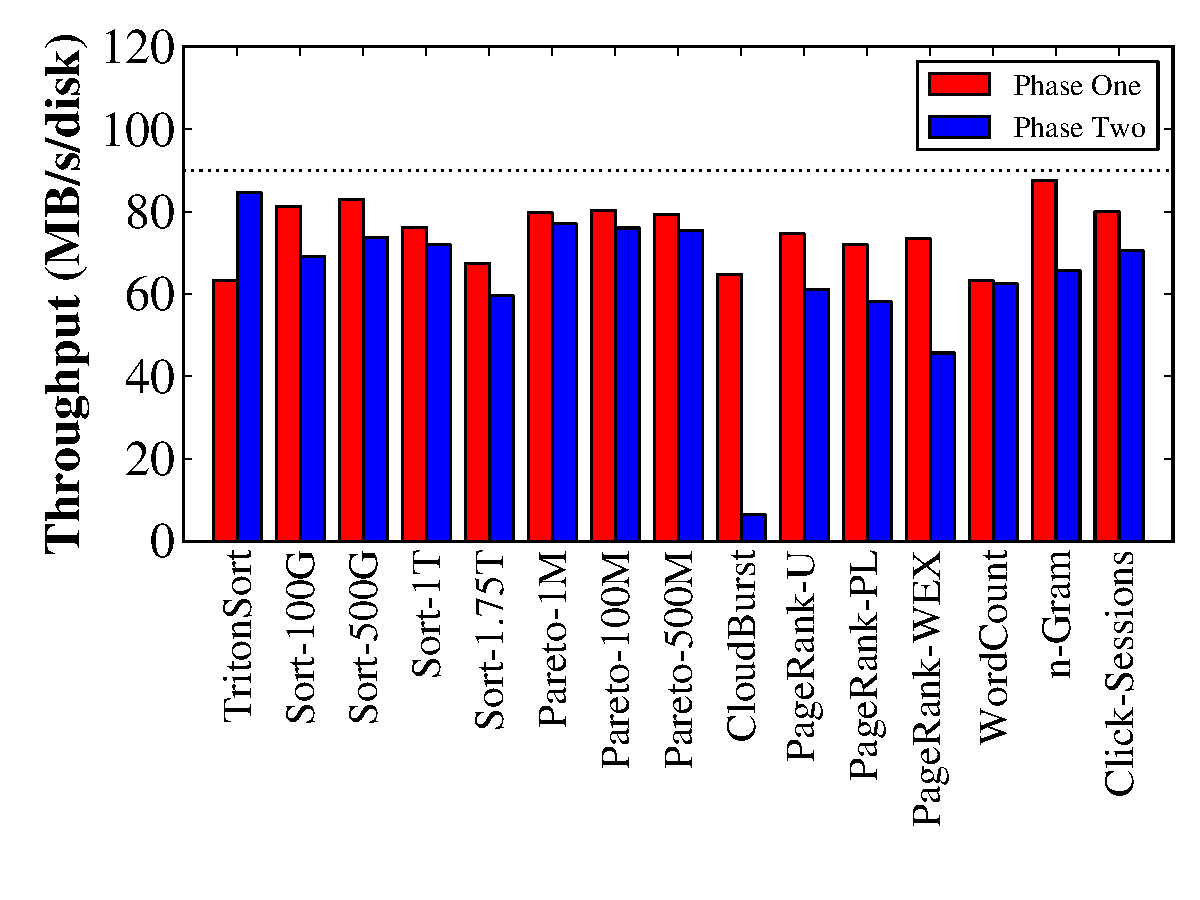
\includegraphics[width=\columnwidth]{themis/graphs/performance.pdf}
\caption{\label{fig:performance} Performance of evaluated MapReduce
  jobs. Maximum sequential disk throughput of approximately 90 MB/s is shown as
  a dotted line. Our TritonSort record from 2011 is shown on the left for
  comparison.}
\end{figure}

The performance of Themis on the benchmark MapReduce jobs is shown in
Figure~\ref{fig:performance}. Performance is measured in terms of
\emph{MB/s/disk} in order to provide a relative comparison to the hardware
limitations of the cluster. The 7200 RPM drives in the cluster are capable of
approximately 90 MB/s/disk of sequential write bandwidth, which is shown as a
dotted line in the figure. A job running at 90 MB/s/disk is processing data as
fast as it can be written to the disks.

Most of the benchmark applications run at near maximum speed in both
phases. CloudBurst's poor performance in phase two is due to the
computationally intensive nature of its \reduce function, which is unable to
process records fast enough to saturate the disks. More CPU cores are needed to
drive computationally intensive applications such as CloudBurst at maximum
speed in both phases. Notice however that CloudBurst is still able to take
advantage of our architecture in phase one.

We have included TritonSort's performance on the Indy 100TB sort benchmark for
reference. TritonSort's 2011 Indy variant runs a much simpler code base than
Themis. We highlight the fact that Themis's additional complexity and
flexibility does not impact its ability to perform well on a variety of
workloads. Our improved performance in phase one relative to TritonSort at
scale is due to a variety of internal improvements and optimizations made to
the codebase in the intervening period, as well as the improved memory
utilization provided by moving from buffer pools to dynamic memory
management. Performance degradation in phase two relative to TritonSort is
mainly due to additional CPU and memory pressure introduced by the \Reducer
stage.

\subsubsection{Comparison with Hadoop}

\begin{table}
  \centering
  \caption{\label{table:hadoop} Performance comparison of Hadoop and Themis.}
  \begin{tabular}{|c|c|c|c|}
    \hline
     & \multicolumn{2}{|c|}{\textbf{Running Time}} &
     \\
    \cline{2-3}
    \textbf{Application} & Hadoop & Themis & \textbf{Improvement}\\
    \hline
    Sort-500G & 28881s & 1789s & 16.14x \\
    CloudBurst & 2878s & 944s & 3.05x \\
    \hline
  \end{tabular}
\end{table}

We evaluate Hadoop version 1.0.3 on the Sort-500G and CloudBurst
applications. We started with a configuration based on the configuration used
by Yahoo! for their 2009 Hadoop sort record~\cite{terasort}. We optimized
Hadoop as best we could, but found it difficult to get it to run many large
parallel transfers without having our nodes blacklisted for running out of
memory.

The total running times for both Hadoop and Themis are given in
Table~\ref{table:hadoop}. I/O-bound jobs such as sort are able to take full
advantage of our architecture, which explains why Themis is more than a factor
of 16 faster. As explained above, CloudBurst is fundamentally compute-bound,
but the performance benefits of the 2-IO property allow the Themis
implementation of CloudBurst to outperform the Hadoop implementation by a
factor of 3.

\subsection{Memory Management}

In this section, we evaluate the performance of our different memory allocation
policies. We also show that our allocation system is robust in the face of
transient changes in individual stage throughputs.

\subsubsection{Memory Allocator Performance}

\begin{figure}
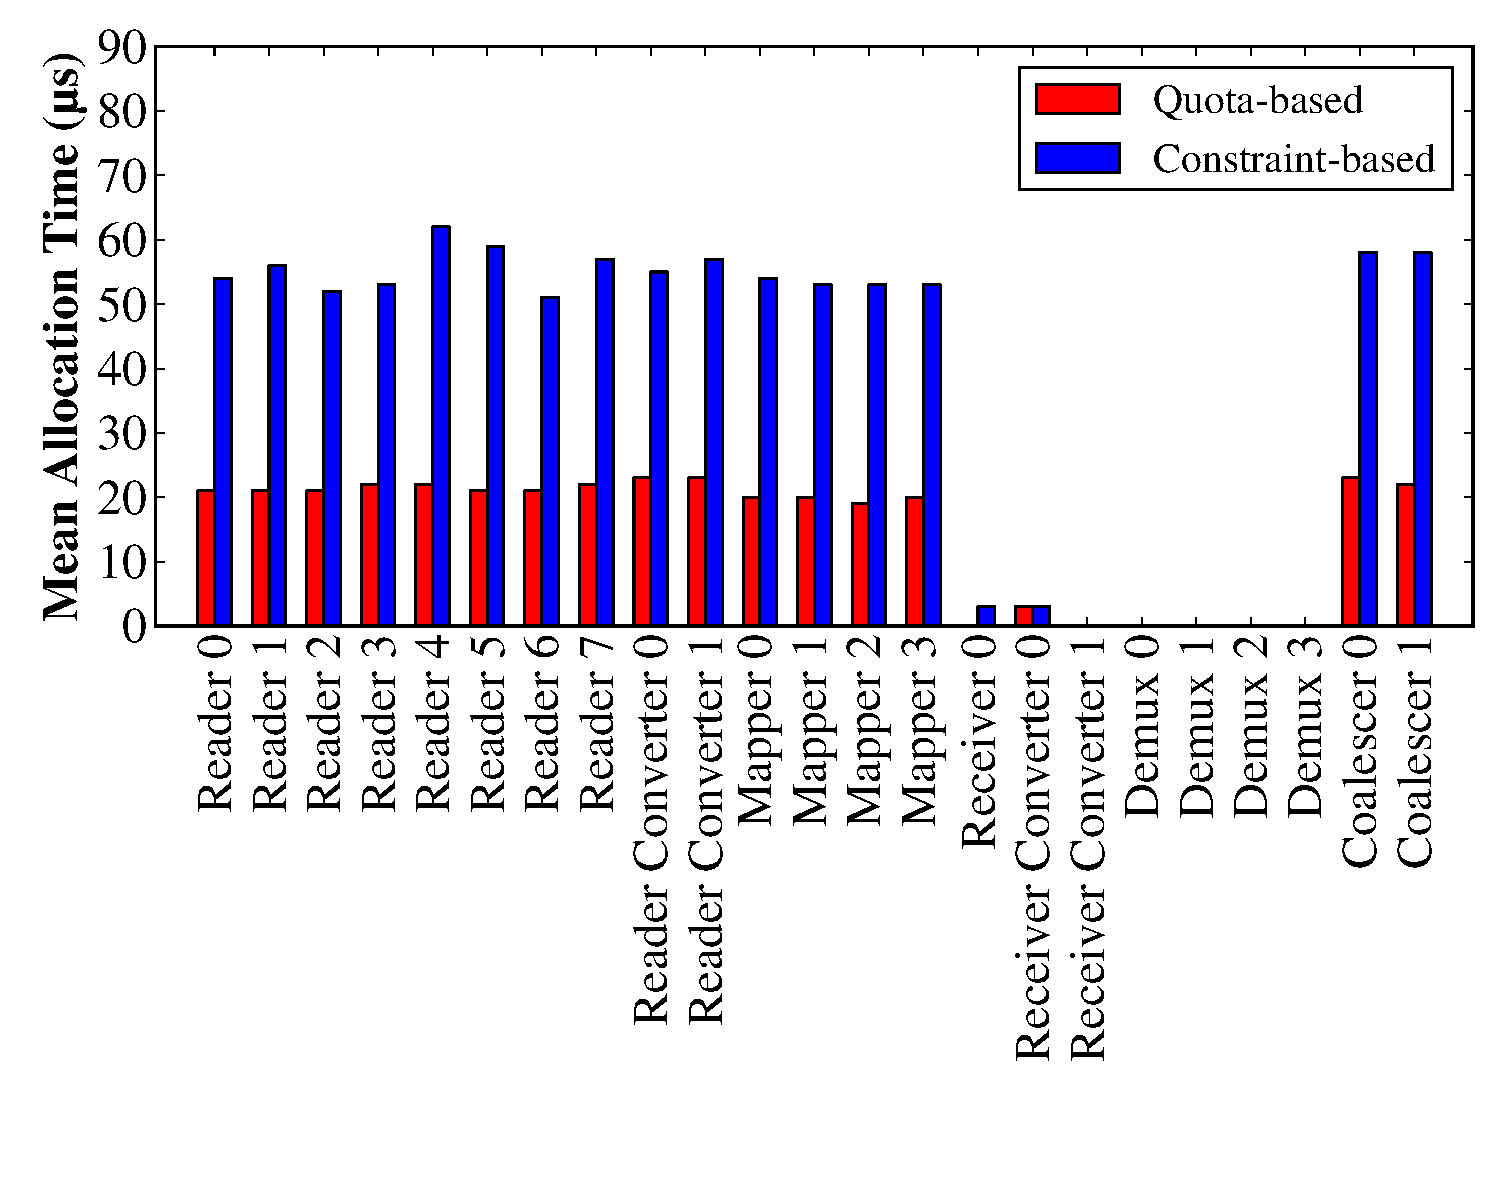
\includegraphics[width=\columnwidth]{themis/graphs/allocation_time_means.pdf}
\caption{\label{fig:allocation_time_means} Effects of allocation policy on mean
allocation times across workers}
\end{figure}

\begin{table}
  \centering
  \caption{\label{table:allocator_end_to_end_performance} Performance of
    allocation policies}
  \begin{tabular}{|c|c|}
    \hline
    \textbf{Allocation Policy} & \textbf{Phase One Throughput} \\
    \hline
    Constraint-Based & 84.90 MBps/disk \\
    Quota-Based & 83.11 MBps/disk \\
    \hline
  \end{tabular}
\end{table}

We examine both the individual allocation times of our different memory
allocation policies and their end-to-end performance.  We evaluate the
performance on phase one of a 200GB, 1-node sort
job. Table~\ref{table:allocator_end_to_end_performance} shows that phase one's
throughput is essentially unaffected by the choice of allocator policy in this
particular instance. These performance numbers can be explained by looking at
the mean allocation time for each worker in the
system. Figure~\ref{fig:allocation_time_means} shows that while the
constraint-based allocator is more than twice as slow as the quota-based
allocator, the absolute allocation times are both measured in tens of
microseconds, which is negligible compared to time taken to actually do useful
work.

However, the results above only hold in the case where the constraint-based
allocator does not deadlock. While we never experienced deadlock in phase two,
we found it was quite easy to construct situations in which phase one
deadlocked. For example, the exact same experiment conducted on a slightly
larger data set causes deadlock in phase one with the constraint-based
allocator.

The performance results in Figure~\ref{fig:performance} demonstrate the
constraint-based allocation policy performs well in phase two.  Because phase
two handles entire intermediate partitions in memory, its allocations are
orders of magnitude larger than those in phase one. This dramatically increases
the likelihood that a single memory request is larger than one of the phase's
quotas.

\subsubsection{Robustness of the Quota-Based Memory Allocation Policy}

\begin{figure}
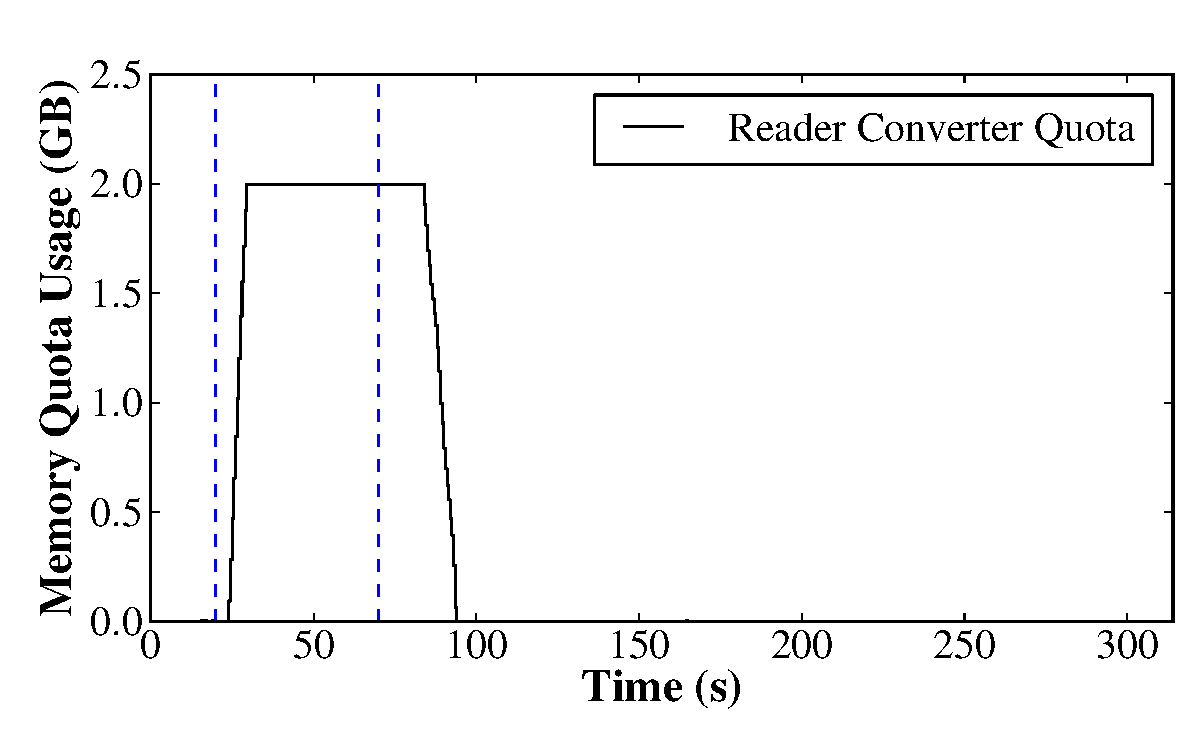
\includegraphics[width=\columnwidth]{themis/graphs/reader_converter_quota_slow_network.pdf}
\caption{\label{fig:reader_converter_quota_slow_network} Memory quota usage of
  the Reader Converter stage. The network was made artificially slow in the
  time period designated by the dashed lines.}
\end{figure}

We evaluate the robustness of the quota-based memory allocator by artificially
slowing down the network for a period of time. We observe the effect on the
total quota usage of a stage in the pipeline. Figure
\ref{fig:reader_converter_quota_slow_network} shows that the Reader Converter's
quota usage spikes up to its limit of 2GB in response to a slow network and
then returns back to a steady state of near 0. A slow network means that stages
upstream of the network are producing data faster than the network can transmit
data. This imbalance leads to data backing up in front of the
network. In the absence of the quota allocation policy, this data backlog grows
unbounded.

\subsection{Skew Mitigation}

\begin{figure}
  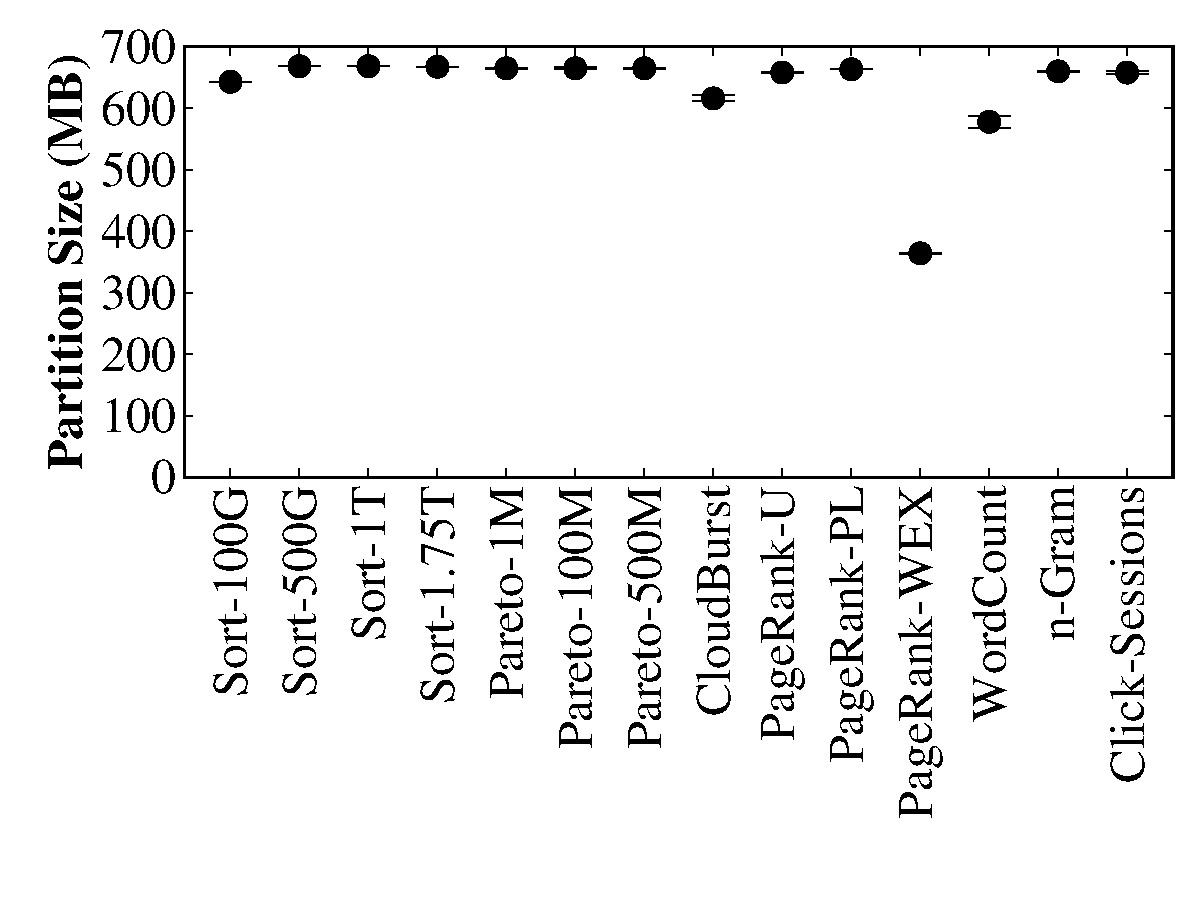
\includegraphics[width=\columnwidth]{themis/graphs/ld_sizes_plot.pdf}
  \caption{\label{fig:ld_sizes} Partition sizes for various Themis
    jobs. Error bars denoting the 95\% confidence intervals are hard to see
    due to even partitioning.}
\end{figure}

Next, we evaluate Themis's ability to handle skew by observing the sizes of
the intermediate data partitions created in phase one.
Figure~\ref{fig:ld_sizes} shows the partition sizes produced by Themis on the
evaluated applications. The error bars denoting the 95\% confidence intervals
are small, indicating that all partitions are nearly equal in size. This is
unsurprising for applications with uniform data, such as sort. However, Themis
also achieves even partitioning on very skewed data sets, such as
Pareto-distributed sort, PageRank, and WordCount. PageRank-WEX has fairly small
partitions relative to the other jobs because its intermediate data size is not
large enough for phase zero to create an integer number of partitions with the
desired size.

\subsection{Write Sizes}

\begin{figure}
  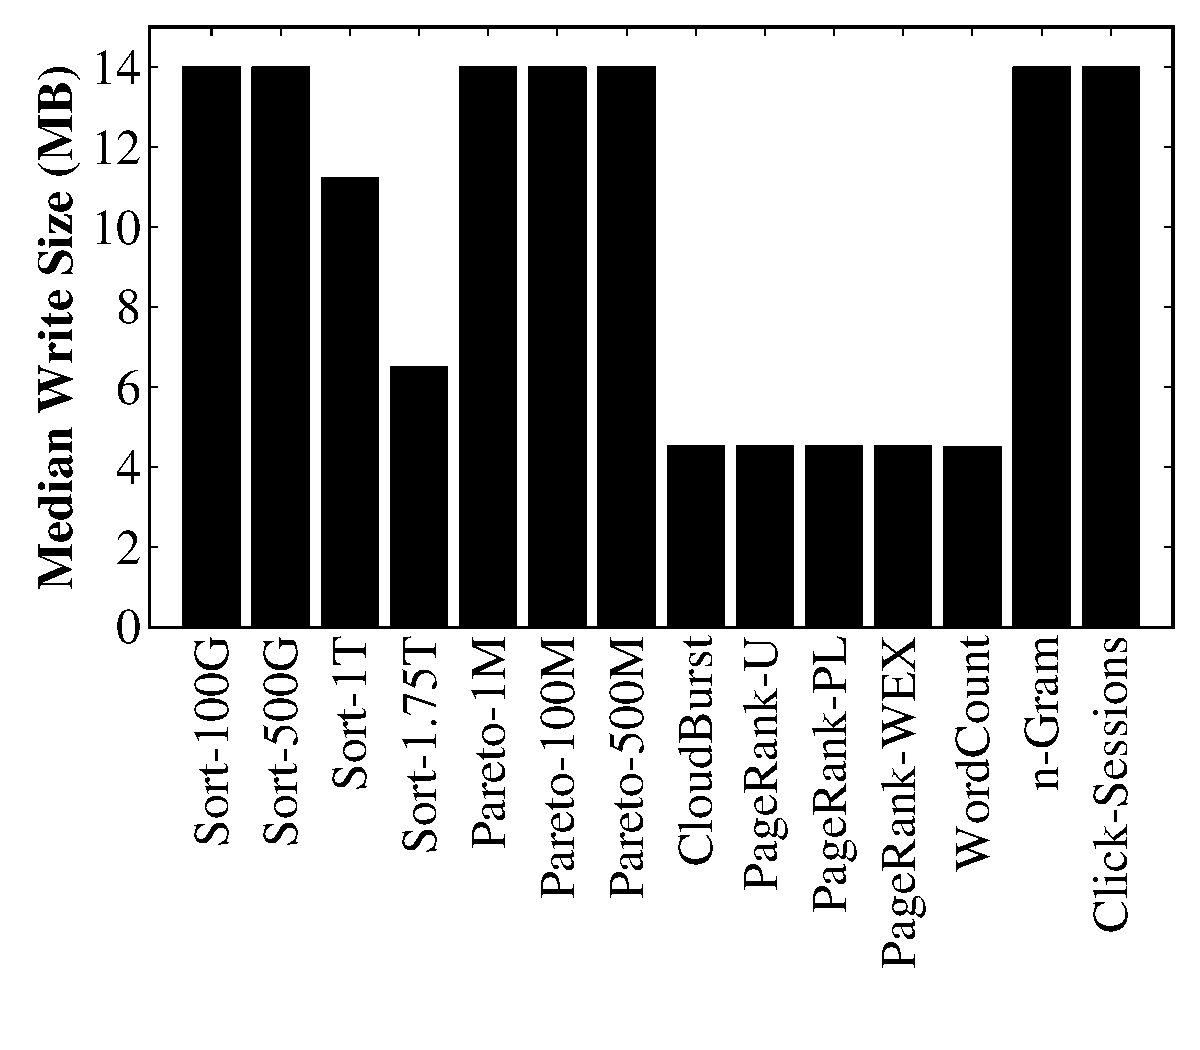
\includegraphics[width=\columnwidth]{themis/graphs/write_sizes_median_bars.pdf}
  \caption{\label{fig:write_sizes} Median write sizes for various Themis jobs}
\end{figure}

One of primary goals of phase one is to do large writes to each partition to
avoid unnecessary disk seeks.  Figure~\ref{fig:write_sizes} shows the median
write sizes of the various jobs we evaluated.  For jobs like Sort and n-Gram
where the \map function is extremely simple and \mappers can map data as fast
as \readers can read it, data buffers up in the \Chainer stage and all writes
are large. As the amount of intermediate data per node grows, the size of a
chain that can be buffered for a given partition decreases, which fundamentally
limits the size of a write. For example, Sort-1.75T writes data to 2832
partitions, which means that its average chain length is not expected to be
longer than about 5 MB given a \receiver memory quota of 14GB; note, however,
that the mean write size is above this minimum value, indicating that the
\writer is able to take advantage of temporary burstiness in activity for
certain partitions.  If the stages before the \Writer stage cannot quite
saturate it (such as in WordCount, CloudBurst and PageRank), chains remain
fairly small. Here the minimum chain size of 4.5 MB ensures that writes are
still reasonably large. In the case of PageRank-WEX, the data size is
too small to cause the chains to ever become very large.

\section{Conclusions}
\label{themis:sec:conclusions}

Many MapReduce jobs are I/O-bound, and so minimizing the number of I/O
operations is critical to improving their performance.  In this work, we
present Themis, a MapReduce implementation that meets the 2-IO property,
meaning that it issues the minimum number of I/O operations for jobs large
enough to exceed memory.  To avoid materializing intermediate results, Themis
foregoes task-level fault tolerance, relying instead on job-level fault
tolerance. Since the 2-IO property prohibits it from spilling records to disk,
Themis must manage memory dynamically and adaptively. To ensure that writes to
disk are large, Themis adopts a centralized, per-node disk scheduler that
batches records produced by different \mappers.

There exist a large and growing number of clusters that can process
petabyte-scale jobs, yet are small enough to experience a qualitatively lower
failure rate than warehouse-scale clusters.  We argue that these deployments
are ideal candidates to adopt more efficient implementations of MapReduce,
which result in higher overall performance than more pessimistic
implementations.  Themis has been able to implement a wide
variety of MapReduce jobs at nearly the sequential speed of the underlying
storage layer, and is on par with TritonSort's record sorting performance.

\section{Acknowledgments}
\label{sec:ack}

The authors wish to thank Kenneth Yocum for his valuable input, as well as
Mehul Shah and Chris Nyberg for their input on Themis's approach to
sampling.  This work was sponsored in part by NSF Grants CSR-1116079 and MRI
CNS-0923523, as well as through donations by Cisco Systems and a NetApp Faculty
Fellowship.

Chapter~\ref{chapter:themis} contains material as it appears in the Proceedings
of the ACM Symposium on Cloud Computing (SoCC) 2012. ``Themis: An I/O-Efficient
MapReduce''. Rasmussen, Alexander; Conley, Michael; Kapoor, Rishi; Lam, Vinh
The; Porter, George; Vahdat, Amin. The dissertation author was the primary
investigator and author of this paper.


